\chapter{Kontejnerizace} 
Kontejnerizace je jeden z typů přístupu k virtualizaci. Nejedná se o klasickou virtualizaci, pomocí které jsou emulovány hardwarové zdroje, ale o tzv. virtualizaci na úrovni operačního systému. Celý princip kontejnerové virtualizace je postaven na izolaci jednotlivých zdrojů operačního systému. Tato virtualizace používá k izolaci systémové zdroje v jádru operačního systému. Na Linuxu se jedná převážně o cgroups, které slouží k izolaci CPU a paměti, pro izolaci procesů pak slouží namespaces. Tento typ virtualizace se stal v posledních letech velmi oblíbený především kvůli své jednoduchosti a rychlosti, a to hlavně díky projektu Docker. S nárůstem popularity kontejnerové virtualizace se začala znovu více používat architektura mikroslužeb.

\section{Historie kontejnerové virtualizace}
I když kontejnery zažívají v posledních třech letech obrovský rozmach, nejedná se zdaleka o nejnovější technologii. První náznaky kontejnerů se objevily během roku 1979, kdy byl do UNIXU v7 naimplementován program chroot \cite{chroot}, který jako jeden z prvních ukázal, jak efektivně izolovat procesy a odlišné souborové systémy. Z UNIXU se chroot dostal na systém BSD v roce 1982. O téměř dvacet let později v roce 2000 se objevil projekt FreeBSD jail \cite{freebsd_jail}, který byl postaven nad konceptem chrootu, rozšiřoval jeho možnosti práce, s procesy a souborovým systémem. Bohužel díky malému rozšíření operačního systému FreeBSD se tento projekt neujal. V roce 2001 byl představen projekt Linux VServer \cite{linux_vserver}, který byl postaven na stejném principu jako předchozí projekt FreeBSD jails. Projekt se sice nestal v komunitě populární, ale je v linuxovém jádře udržován dodnes. V roce 2004 se kontejnerovou virtualizací začala zabývat také firma Oracle, která ve svém operačním systému Solaris vytvořila projekt Solaris Containers často označován jako Solaris Zones \cite{solaris_zones}. Celý projekt byl postaven nad konceptem zón, pomocí kterých byla tvořena jednotlivá separace. Mezi roky 2004-2008 se pokoušela spousta projektů prorazit se svým kontejnerovým konceptem. Hlavními hráči zde byly OpenVZ. Jednalo se o projekt, který byl opět postaven na linuxovém jádru \cite{openvz}. Ovšem zdrojové kódy které pro své řešení použili, se nikdy oficiálně nedostaly do linuxového jádra, bylo nutno tedy jádro patchovat. Další projekt Process Containers, byl vytvořen společností Google a byl opět postavený na linuxovém jádře. V roce 2007 byl tento projekt oficiálně přejmenován na control groups (cgroups) \cite{pc_cgroups}, převážně kvůli dvojsmyslu slova kontejner, které bylo použito v předchozím názvu. Tato změna byla přidána do linuxového jádra během roku 2007 a v lednu roku 2008 byl projekt oficiálně zahrnut do verze jádra 2.6.24. Projekt Process Contraines určil směr, jak by měla izolace procesů v linuxovém jádře vypadat. Ve stejném roce se objevil projekt LXC (LinuX Containers) \cite{lxc}, kterým byla první kompletní lehkotonážní technologie zaměřená na správu kontejnerů. Technologie byla postavená nad cgroupami a namespaces a přidána do linuxového jádra, takže pro svůj běh nebylo třeba žádných externích změn. V roce 2013 se na kontejnerovou scénu opět vrací Google, který otevřel zdrojové kódy ke svému kontejnerovému řešení zvanému Let Me Contain That For You (LMCTFY) \cite{lmctfy}. Cílem tohoto projektu bylo poskytnout abstrakci na kontejnery a možnost spravovat je skrze API. V roce 2015 bylo rozhodnuto, že veškerá logika a koncepty tohoto projektu budou sloučeny s projektem Docker a knihovnou libcontainer, kterou Docker používal. Samotný Docker projekt, který masově rozšířil kontejnerovou virtualizaci a nastartoval tak novou éru vývoje softwaru, vznikl jako projekt Solomona Hykese, který tento projekt vytvořil ve firmě dotCloud. Firma posléze převzala projekt za svůj, změnila svoje jméno na Docker a začala se věnovat pouze této technologii a orchestraci okolo ní \cite{docker_rename}. Docker se stal standardem a vybudoval si téměř monopol. V následujících letech se začala objevovat další řešení jako například, rkt od firmy CoreOS (dnešní Red Hat), která vyvinula svůj systém kontejnerů. Rkt fungoval i jako runtime a dokázal spouštět i Docker kontejnery. Volba na tvorbu vlastního kontejner enginu se nezrealizovala díky dlouhému čekání na schvalování patchů do Docker projektu. V roce 2015 pak vznikla organizace Open Container Initiative (OCi) \cite{OCI_standard}, která nastavila a popsala standard pro kontejnery. Snahou bylo mít kontejnery univerzální s možností jednoduché změny jednotlivých řešení. S rozmachem ochestrátoru Kubernetes se začaly v roce 2017 objevovat kontejnery a runtime určené pouze pro tento orchestrátor, jednalo se o projekty jako např. Containerd a Podman. Ve stejném roce Docker oznámil, že bude také přispívat do Kubernetes a nebude upřednostňovat pouze svůj orchestrátor Swarm. Během nadcházejícího roku se Kubernetes stal populárním tak, že ho do svých produktů zařadily všechny tři hlavní firmy působící v oblasti veřejného cloudu (Azure, Amazon a Google).

\section{Kontejnery}
Princip kontejnerů a kontejnerové virtualizace je založen na izolaci jednotlivých částí aplikace na sobě nezávisle fungujících celků. Pro svůj běh kontejnery používají izolované zdroje, jako jsou CPU, disk nebo síť, pomocí kterých je kontejner oddělen od zbytku systému. Kontejner si lze velmi jednoduše představit jako klasický kontejner na přepravu zboží. Je vždy uzavřen a měl by fungovat sám o sobě. Do kontejneru lze velmi jednoduše zabalit nainstalované aplikace i s jejich podpůrnými knihovnami a nastavením, celé kontejnery pak lze velmi snadno přenášet mezi různými prostředími.

Obrovskou výhodou kontejnerů je možnost spuštění několika stejných služeb, jako jsou například databáze, v jednom prostředí bez možnosti, aby se služby navzájem ovlivňovaly. Další výhodou je bezpečnost veškerých akcí, které jsou spuštěny v kontejneru. Akce jsou odděleny od operačního systému hosta. Kontejnery také řeší aplikační problém se závislostmi. Díky kontejnerovému řešení lze nainstalovat potřebné balíčky a knihovny přímo do kontejneru. Je tedy možné aplikaci v produkčním nastavení vyzkoušet přímo na stroji, na kterém je aplikace vyvíjena. Tato skutečnost značně zjednodušuje práci vývojářům, kteří si mohou velmi snadno a rychle otestovat svou aplikaci. Obdobně pomáhá při práci administrátorům, kteří se nemusí bát o zpětnou kompatibilitu a nestabilitu aplikace.

Kontejnery bývají často srovnávány s klasickými virtuálními stroji. Ovšem jedná se o úplně jiný princip virtualizace. V kontejneru by měl být spuštěn pouze jeden proces jako PID 1. Oproti plně virtualizovaném serveru, kde je proces PID 1 init nebo systemd, který má další procesy jako své potomky. Z tohoto důvodu je spuštění virtuálního stroje mnohem pomalejší a může trvat řádově v minutách, naopak spuštění kontejneru je záležitostí několika vteřin. Další výhodou kontejnerového přístupu je práce se zdroji, kontejner dokáže ke zdrojům přistupovat dynamicky na rozdíl od virtuálního stroje, který si musí před svým startem zdroje předalokovat, tyto změny poté většinou nelze jednoduše upravovat. Chybné počáteční nastavení zdroje pro virtuální stroj může mít negativní vliv na alokované zdroje, které reálně nikdy nevyužije. Díky tomuto principu jsou virtuální stroje vhodnější pro jiný typ workloadu než kontejner, například pro stavové aplikace, kde je dopředu zřejmé, jaké zdroje bude aplikace potřebovat. Při použití virtuálních strojů je spuštěn nový operační systém s vlastním jádrem. Ten je mnohem jednodušší zabezpečit \cite{vm_container}. Na druhé straně ve světě virtuálních strojů existuje stále ještě řada problémů, např. řešení vysoké dostupnosti aplikací nebo řešení konfigurace virtuálních strojů a jejich škálování.

\begin{table}[H]
\begin{center}
\caption{Porovnání kontejneru a VM} 
\label{tbl:orch_comp}
\begin{tabular}{|p{25mm}|p{55mm}|p{55mm}|}
\hline
  ~   & Virtuální stroje (VM) & Kontejnery \\    \hline
Velikost: &  Velká &  Nízká  \\    \hline
Škálovatelnost: &  Pomalá - nutnost škálovat celé virtuální stroje &  Rychlá - škálované jsou pouze kontejnery \\    \hline
Nasazení: & Pomalé - nasazení vyžaduje nastavit aplikaci a operační systém & Rychlé - aplikace již je nainstalována v images, které jsou spouštěny \\    \hline
Izolace: &  Úrovni systému & Úrovni procesu  \\    \hline
Přenositelnost: & Nižší & Vysoká \\    \hline
Granularita komponent: & Vysoká & Nízká  \\    \hline
Bezpečnost: & Vysoká & Nízká  \\    \hline
\end{tabular}
\end{center}
\end{table}

Pro kontejnerizaci existuje velké množství technologií, nejznámější z nich je Docker. Docker přišel s jednoduchým a srozumitelným konceptem pro snadné používání kontejnerů. Docker ovšem není jediná dostupná kontejnerová technologie. Do vývoje Dockeru se snažili přispívat vývojáři nejen z firmy Docker, ale i z jiných firem. Proto vznikaly nové projekty, např. projekt rkt od firmy CoreOS, který se technologií Docker nechal velmi inspirovat. Tento projekt se ve srovnání s Dockerem zaměřoval na bezpečnost, zároveň byl s Dockerem kompatibilní, to znamená, že v rkt prostředí bylo možno též spouštět image vytvořené pro Docker. Během roku 2015 byla založena iniciativa OCi, která měla za úkol standardizovat svět kontejnerů. Zakládající členové byly společnosti Docker a CoreOS. Hlavní standardy, které jsou uveřejněny pod OCi, jsou standardy pro image a runtime \cite{OCI_standard}. Image standard popisuje, jak by měla vypadat image, ze které je možné spustit kontejner. Runtime popisuje, jak má být kontejner spuštěn a jak má vypadat jeho životní cyklus. Tyto dva standardy otevřely cestu projektům, jako jsou Crio-O a podman, které byly převážně vyvíjené společností Red Hat, která se snažila kolem kontejnerů postavit svůj vlastní business. Zajímavostí je, že podle zdroje \cite{redhat_docker} Red Hat byl již v roce 2016 v kontejnerovém businessu finančně mnohem úspěšnější a dokázal na technologii Docker vydělat mnohem více peněz než právě firma Docker. Od začátku bylo cílem Red Hatu dostat Docker ze svých produktů úplně, aby měl nad svými produkty větší kontrolu. V současnosti již je možné vytvářet a spouštět kontejnery bez použití technologie Docker.

Z průzkumů prováděného zdroji \cite{sysdig_survey} a \cite{hq_survey} vyplývá, že nejrozšířenější a nejpoužívanější kontejnerizační řešení je Docker. Architektura Docker kontejneru je postavena na systému vrstev. Každá vrstva vždy obsahuje pouze data z akce, která byla na dané vrstvě vykonána. Všechny vrstvy kromě nejvyšší (tzv. kontejnerovou vrstvy) jsou v režimu Read-Only, to znamená, že do těchto vrstev není možno zapisovat data, ale pouze z nich číst. Veškeré akce, které jsou prováděny v kontejneru po jeho spuštění, probíhají v kontejnerové vrstvě. Tento vrstvový systém lze použít díky unionFS \cite{unionfs}, speciálnímu typu souborového systému, který Docker využívá. Pro tvorbu jednotlivých kontejnerů se používají takzvané Docker image. Image je předpis jenž obsahují aplikaci se všemi závislostmi na spuštění, například MySQL, Redis nebo runtime pro programovací jazyky (JRE, Node). Prostřednictvím těchto imags se poté distribuují jednotlivé kontejnery. Jedná se o samostatnou spustitelnou jednotku, která obsahuje aplikaci nebo část aplikace i s jejími závislostmi. Pokud je potřeba vytvořit vlastní image, lze to pomocí speciálního souboru zvaného Dockerfile.

\begin{lstlisting}[caption={Dockerfile, zdroj: vlastní tvorba},label={lst:dockerfile}]
FROM openjdk:8-jre-alpine3.8

COPY ./target/file-service.jar /app/
RUN mkdir /filevol
RUN mkdir /logs
CMD ["java", "-Xmx200m", "-jar", "/app/file-service.jar"]

EXPOSE 7000
\end{lstlisting}

Základní stavebním kamenem Docker, jak již bylo zmíněno, je Dockerfile, jehož strukturu lze vidět v ukázce kód \ref{lst:dockerfile}. Jedná se o textový soubor, který má pomocí klíčových slov provádět akce potřebné k sestavení image. Každý Dockerfile začíná klíčovým slovem \textit{FROM}, které specifikuje základní image, ze které se vychází. Hlavním požadavkem na tyto image je především malá velikost a potřeba dávat do kontejnerů pouze data nezbytně nutná pro jejich běh. Jako základní image pro kontejnery se často využívá Alpine Linux, což je lehkotonážní linuxová distribuce, která má v základní verzi pouze 5 Mb \cite{docker_alpine}. Tato distribuce je zúžena o všechny nepotřebné knihovny a nástroje. Ve zmiňované ukázce je použit Alpine, který má již v sobě předinstalované prostředí pro spouštění jar souborů. Tato image pochází z repozitáře Docker Hub, jenž je nejpopulárnějším repozitářem pro Docker image. Ve druhém kroku pomocí příkazu \textit{COPY} dojde k překopírování souborů z lokálního souborového systému do image. V příkladu je nakopírován jar balíčku obsahující aplikaci. Jako další je použito klíčové slovo \textit{RUN}, které slouží ke spouštění různých shellových příkazů, v příkladu je pomocí něho volán příkaz mkdir, který vytváří adresáře vyžadované aplikací. V praxi se tento příklad často používá na instalaci balíčků z repozitářů jednotlivých linuxových distribucí. Předposlední příkaz \textit{CMD} určuje, jak bude probíhat start kontejneru, v příkladu pak spouští překopírovaný jar soubor pomocí JRE. Pokud je nutné pro aplikaci před spuštěním vykonat nějakou složitější logiku, například zkontrolovat práva na souborech v kontejneru či připravit aplikaci (např. dokonfigurovat), tak se používá příkaz \textit{ENTRYPOINT}. Entrypoint dává možnost ještě před startem spustit shellový skript s přidanou logikou. Poslední příkaz \textit{EXPOSE} poté slouží k určení, na jakém portu bude aplikace vystavena. V příkladu je použit port 7000. Dále lze specifikovat i protokol, který bude ke komunikaci použit. Je možné vybrat z tcp nebo udp, ale pokud protokol není nadefinován, je vždy vybrán tcp. Image lze pak sestavit dvěma různými způsoby. První je pomocí Docker CLI a příkazem \textit{docker build .}, druhý pomocí orchestátoru Compose. Jak už bylo zmíněno výše, image jsou ukládány a přenášeny pomocí repozitářů, výchozí je Docker Hub. Práce s repozitářem je velmi jednoduchá, pracuje se s ním také pomocí Docker CLI a struktura příkazů je značně podobná verzovacímu systému Git.

\section{Mikroslužby}
Princip architektury mikroslužeb (Microservices) je velmi podobný Unixové filozofii, která vychází z konceptu mnoha malých jednoúčelových programů, kde každý vykonává pouze jednu činnost, zato spolehlivě. Z praktického hlediska to znamená, že aplikace, která používá princip mikroslužeb, by měla být rozdělena do jednotlivých zapouzdřených komponent, které vždy vykonávají pouze jednu akci. V rámci webové aplikace to může být například služba na přihlášení či vyhledávání. Základní rozdíl mezi mikroslužbami a monolitickým přístupem je dělení aplikace na jednotlivé části. Aplikace jsou lehce uchopitelné, mnohem lehce spravovatelné a nezávislé. Služby by měly být maximálně nezávislé, ať už se jedná o jejich zdrojový kód, nebo o možnost nasazení \cite{microservices1}. Jednotlivé služby by měly být navrženy tak, aby bylo možné jejich nové verze nasazovat a testovat nezávisle na ostatních službách, se kterými jsou propojeny. S konceptem mikroslužeb je nutné veškeré procesy automatizovat, protože se velmi jednoduše může stát, že počet jednotlivých mikroslužeb bude velmi rychle narůstat. Důležité je mít pod kontrolou jejich nasazování, testování a hlavně monitoring \cite{microservices2}. Jednotlivé služby mohou být nasazovány i nezávisle a při nasazení může i malá chyba v jedné službě způsobit globální problém v celé aplikaci. V chybně navržené architektuře může i chyba jedné služby způsobit výpadek celé aplikace. Proto je nutné jednotlivé komponenty držet co nejvíce izolované. Dále je nutné na celé řešení pohlížet jako na decentralizovaný systém, kde by v ideálních podmínkách výpadek jedné služby neměl ovlivnit zbytek. Často nebývá tento koncept pochopen správně a bývá pro všechny mikroslužby používána jedna databáze. V ideálním případě je nutné databáze rozdělit tak, aby mohly být lépe decentralizované, což bývá často problematické, protože je nutno zachovat jednotlivé vazby mezi databázemi. K dalším nevýhodám přístupu mikroslužeb patří problémy s API, obtížnost architektury aplikace a jednotlivé ovlivňování mikroslužeb navzájem. Čím víc se API dané mikroslužby používá, tím obtížnější je ho změnit. Nekompatibilní změna do API poté ovlivní veškeré další mikroslužby. Dalším problémem je často chybný návrh architektury. Architektura mikroslužeb není vhodná pro všechny typy aplikací. Především pro menší systémy, které nepotřebují dynamické škálování, je stále vhodnější monolitická architektura. I když svět mikroslužeb není zcela dokonalý, výhody převyšují. Velkou výhodou výsledku vývoje aplikace je jednoduchost, izolovatelnost, testování, vlastnictví a škálovatelnost. Aplikace postavené na konceptu mikroslužeb se výrazně lépe škálují, lze u nich škálovat i pouze jednotlivé části. Viz schéma architektury mikroslužeb na obrázku \ref{fig:mikrosluzby}.

\begin{figure}[H]
\begin{centering}
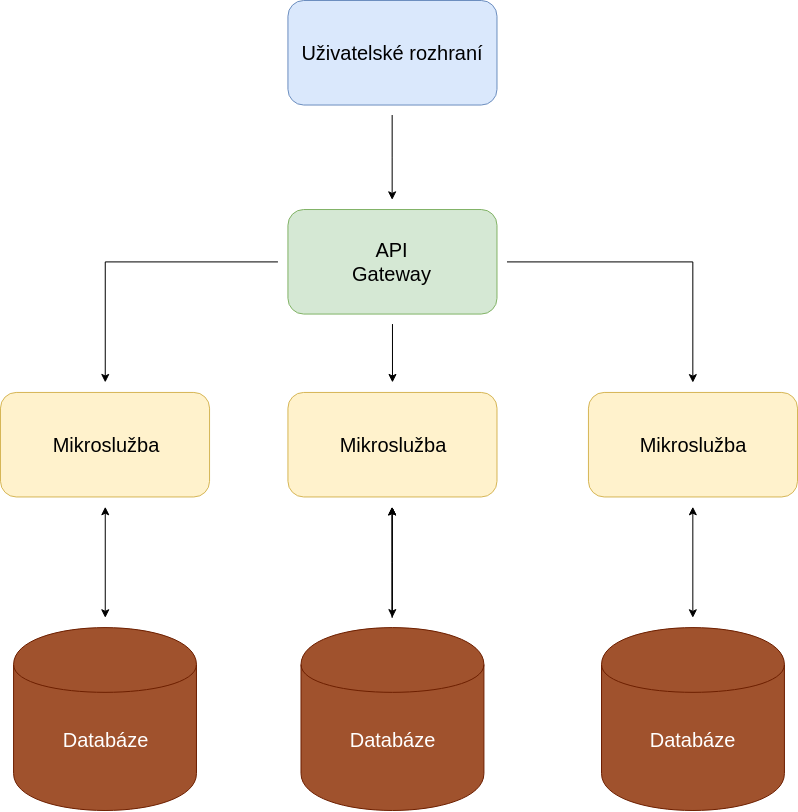
\includegraphics[width=0.8\textwidth]{img/mikrosluzby.png}
\par\end{centering}
\caption{Schéma mikroslužeb, zdroj: vlastní tvorba} \label{fig:mikrosluzby}
\end{figure}

\section{Orchestrátory}
Hlavní problém v kontejnerové virtualizaci byla správa a lifecycle management (LCM) samotných kontejnerů. Jelikož kontejnerová aplikace bývá často složena z několika desítek kontejnerů, je nutné proces správy automatizovat co nejvíce, protože není možné jednoduše řídit kontejnerové aplikace ručně. Bylo nutno vyřešit, jak naimplementovat orchestrační vrstvu nad kontejnerovým řešením. Na kontejnery byl kladen požadavek na vyšší abstrakci nad jednotlivými zdroji za účelem zjednodušení principu ovládání a nastavování oproti klasickým virtuálním strojům. Důraz byl kladen především na networking, aby komunikace mezi jednotlivými kontejnery probíhala pouze přes DNS jména, která lze naimplementovat pomocí DNS záznamů. Záznamy slouží ke zjednodušení práce vývojářů, kteří pak nemusí složitě řešit síťové problémy. Dalším důvodem pro používání orchestrátorů je spojování kontejnerů do vyšších logických prvků. Například databázi je často vhodné spouštět spolu sdané databázovou cache. Takže při škálování dané komponenty je služba škálována také s podpůrnou službou. Dále vznikla potřeba orchestrovat i stavové aplikace. Je tedy potřeba vyřešit problém připojování svazků dat do příslušných kontejnerů. A to nejen při běhu, ale také při výpadku kontejneru.

V orchestrátoru lze odlišit dva základní termíny, a to orchestrace a scheduling. Scheduling je algoritmus zodpovědný za spouštění kontejnerů a orchestrace slouží k jejich řízení. Scheduler vždy bývá implementován jako součást orchestrátoru a zajišťuje rovnoměrné spouštění kontejnerů po hypervisorech a má přehled o zdrojích, které a kde spustit. Scheduler by měl fungovat i v rámci disaster recovery scénáře. Pokud se na hypervisoru vyskytne chyba, scheduler to zjistí a automaticky spustí kontejnery na jiném serveru. Orchestrace dále zajišťuje konzistenci v clusteru a sleduje počet kontejnerů. Pokud v clusteru nějaký chybí, tak spustí nový, pokud přebývá, tak ho zastaví. Z výše uvedených důvodů vyplývá, že ve velkém aplikačním clusteru provoz kontejnerů bez orchestrátoru nemůže fungovat. Samotný kontejner je pouze stavební jednotka většího celku. Stejný problém řešila i firma Google, která s kontejnery experimentovala ještě před kontejnerovým boomem v roce 2014. Podle zdroje \cite{google_container} již v roce 2014 bylo v Googlu spouštěno každý týden přes dvě miliardy kontejnerů, proto se společnost Google rozhodla vybudovat vlastní systém na orchestraci kontejnerů zvaný Borg. V současné době firma Google provozuje své veškeré aplikace v kontejnerech.

\section{Stavové a bezstavové aplikace}
S orchestátory a kontejnery přichází další problém, který bylo potřeba vyřešit, a tím jsou stavové aplikace. Stavové aplikace jsou typ aplikací, které si pro svůj běh potřebují držet data. Může se jednat například o databáze, které drží data pro webový backend. Data v databázích jsou průběžně aktualizována se změnami ve webové aplikaci, proto je důležité tato data perzistentně ukládat mimo kontejner, aby nedošlo k jejich ztrátě. Kontejnery by měly být bezstavové a jít jednoduše restartovat či převytvořit bez jakékoliv ztráty dat. Oproti stavovým aplikacím jsou postaveny bezstavové aplikace, které si žádný aktuální stav nedrží, pracují s daty, které si aplikace bere z externího API. Obvykle jsou závislé na datech třetích stran, která nejsou uložena v aplikaci. Bezstavová aplikace tedy není závislá na žádných datech uložených v aplikaci. Tento fakt dává bezstavovým aplikacím ohromnou výhodu, dají se velmi rychle a efektivně horizontálně škálovat bez zásahu do aplikace. Dále lze velmi efektivně provádět rollbacky aplikace. Bezstavové aplikace jsou mnohem lépe udržovatelné, což je velmi výhodné v kombinaci s architekturou mikroslužeb a kontejnerovým přístupem.

\section{Porovnání orchestrátorů}
Před porovnáním orchestrátorů je nutné představit ty nejpoužívanější. Je potřeba zmínit, že v současnosti všechny nástroje okolo kontejnerové virtualizace, ať už se jedná o orchestrátory, runtime či kontejnery samotné, jsou open source a jsou dostupné zdarma.

\subsection{Docker orchestrátory}
I samotná firma Docker zjistila, že provoz kontejnerů a kontejnerových aplikací bez orchestrátorů je velmi obtížný. Proto se rozhodla vytvořit hned dvě řešení, pomocí kterých je možné kontejnery ovládat. Prvním řešením je Docker Compose, tento nástroj není oficiálně označován Dockerem jako orchestrátor a splňuje nadefinované požadavky pro orchestrátory. Tento projekt je oproti ostatním velmi jednoduchý, nemá žádnou složitou architekturu, skládá se pouze z jednoho binárního souboru, pomocí kterého jsou spouštěny Compose soubory. Compose soubor je dokument ve formátu yaml, ve kterém je popsané, jak by daná kontejnerová aplikace měla být vytvořena a jak by jednotlivé zdroje měla používat (volumes, síťové porty). Z Compose definice lze též přímo volat sestavování souboru Dockerfile. Compose díky své jednoduchosti není určen pro běh kontejneru na produkci, ale slouží primárně pro vývojáře, kteří si s jeho pomocí jsou schopni spustit vyvíjenou aplikaci. Často také bývá Compose, díky své rychlosti, zaintegrován do testovacích prostředí.

\begin{lstlisting}[caption={Docker Compose, zdroj: vlastní},label={lst:compose_file}]
version: '3'
services:
  database:
    image: mysql
    restart: always
    ports:
    - 3306:3306
    - 33060:33060
    volumes:
      - ./data:/var/lib/mysql
    environment:
      MYSQL_ROOT_PASSWORD: password
\end{lstlisting}

Ukázku Compose souboru je možno vidět na ukázce kódu číslo \ref{lst:compose_file}. Compose musí začínat verzí Composu, poté je vždy definován blok služeb, pod kterým jsou nadefinované jednotlivé komponenty aplikace a jejich vlastnosti. V příkladu je pro demonstraci použita databázová aplikace MySQL. Je specifikováno, že jako image je využita MySQL, restart určuje, kdy se má kontejner restartovat. Pod ports je specifikován list portu a na jaké hosty porta mají být namapovány. V příkladu jsou použity stejné porty jak pro hosta, tak pro kontejnerovou aplikaci. Volumes specifikují část kontejneru, která má ukládat své soubory na souborový systém hosta. V příkladu je namapovaná cesta \textit{/var/lib/mysql}, ve které jsou uloženy data databáze. Takže při použití nejsou data z kontejneru databáze po restartu ztracena. Poslední část aplikační definice tvoří environmentální proměnné, které slouží pro konfiguraci samotné aplikace. Jediná proměnná, kterou je nutné definovat, aby se databáze spustila, je \textit{MYSQL\_ROOT\_PASSWORD}, což je heslo pro uživatele root.

Druhým řešením je Docker Swarm. Jak již název napovídá, projekt se zaměřuje na orchestraci kontejnerů a byl vytvořen společností Docker. Na rozdíl od Docker Compose se Swarm zaměřuje na běh kontejnerových aplikací v produkčních prostředích. Je složitější a obsahuje spoustu důležitých vlastností, které Compose nemá, jako jsou například škálování, load balancing atd. Architektura Swarm clusteru je rozdělena na dvě základní komponenty, a to na workers nody a managers nody. Workers nody slouží k provozu kontejnerů a managery pak pro jejich správu. Jednotlivé role se dají kombinovat. Server může obsahovat manager i worker roli zároveň. Pouze přes manager lze přistupovat do clusteru a spouštět v něm jednotlivé příkazy přes Docker CLI. Manager zajišťuje dále několik rolí: scheduling (spouštění kontejnerů), škálování, health check, DNS a networking. Bezpochyby největší výhodou tohoto řešení je jeho provázanost s Docker ekosystémem. Swarm orchestrátor lze velmi rychle a lehce nainstalovat a spravovat. Samotná instalace probíhá pomocí docker-enginu, Swarm je totiž součástí instalačního balíčku s Dockerem. Jednotlivé produkty se dají jednoduše spojovat a ovládat. Například pomocí Docker Compose lze spouštět předdefinované compose soubory přímo ve Swarmu \cite{swarm_compose}.

\subsection{Kubernetes}
Dalším vybraným orchestátorem je Kubernetes (zkráceně k8s), tento nástroj byl vytvořen Joe Bedou \cite{k8s_beda_commit} za jeho působení ve firmě Google. Předlohou pro tento nástroj byl interní Google orchestrátor zvaný Borg. K8s je také jediný z orchestátorů, který je členem CNCF (Cloud Native Computing Foundation), tato organizace spolu s velkou vývojářskou otevřeností vybudovala okolo tohoto orcherstátoru obrovskou uživatelskou komunitu. Komunita měla značný vliv na celkový rozvoj orchestrátoru. K8s je velmi modulární a nabízí hned několik výměnných modulů ať pro síťové řešení (CNI - Container Network Interface), nebo pro storage (CSI - Container Storage Interface). V k8s clusteru jsou servery rozděleny do dvou skupin, master a minion. Master je složen z několika komponent, hlavní z nich je API server, který slouží ke komunikaci. API je využíváno například k8s CLI klientem, další komponenta je Etcd, key-value databáze, která si ukládá aktuální stav clusteru, dále je zde manager se schedulerem, které zajišťují spouštění a běh kontejnerů. Na straně miniona se nachází kube-proxy, který spravuje networking pro pody, a kubelet služba, která slouží k propojení miniona s api serverem. Nad těmito základními komponentami jsou spouštěny k8s objekty. Základní jednotkou v k8s není jednotlivý kontejner, ale pod. Pod je logická jednotka složená z kontejnerů, tyto pody určují logické celky, které jsou poté spolu škálovány (např webová aplikace a cache). Daný pod je bezstavový, je spouštěn vždy na jednom serveru, kontejnery v něm sdílejí síťové zdroje, IP adresu a komunikují mezi sebou pomocí portu. Do kontejnerů lze také připojovat volume s daty. Jednotlivé pody jsou provázány pomocí k8s služeb, které zajišťují nejen komunikaci uvnitř clusteru, ale je možno pomocí loadbalanceru a ingress služby vystavit také mimo cluster do internetu. Pro stavové aplikace je v k8s objekt statefulset, který má při vytvoření nadefinovaný datový volume s cestou, do které se připojí. Volume je perzistentní, to znamená, že při ztrátě či smazání kontejneru spuštěného statefulsetu nebude smazán. Pro spuštění nových kontejnerů a škálování slouží komponenta replica set (dříve replication controller), která sleduje aktuální počet kontejnerů v clusteru a ukládá si stav do Etcd. Pokud nějaký server s kontejnery postihne výpadek, tak to replicaset zjistí a spustí kontejnery, které byly ztraceny na jiném serveru. Jednotlivé aplikace jsou v k8s odděleny pomocí namespaces. Namespace si lze představit jako další virtuální cluster, ve kterém pody mohou komunikovat pouze v rámci namespace. K identifikování objektů v clusteru slouží label, ty ve formátu klíč–hodnota slouží k popisování a propojování objektů. Jednotlivé definice s objekty jsou pro k8s nadefinované prostřednictvím takzvaných manifestů. Manifest je soubor ve formátu yaml, ve kterém jsou blokově definovány jednotlivé objekty. Díky popularitě v komunitě se k8s stal standardem na poli kontejnerové virtualizace a rozšířil se do většiny velkých firem. Pro běh clusteru totiž není potřeba žádný dedikovaný tým, jak tomu většinou je u privátního cloudu, kdy jeden tým zajišťuje podporu pro ostatní vývojáře. V k8s bylo celé řešení navrhováno tak, aby fungovalo out-of-box (bez zásahu z venku) s cílem, aby se vývojáři mohli soustředit pouze na vývoj aplikací a nikoliv na infrastrukturu.

\begin{lstlisting}[caption={Kubernetes Manifest - Nginx deployment, zdroj: \cite{k8s_docs_deployment}},label={lst:nginx_deployment}]
apiVersion: apps/v1
kind: Deployment
metadata:
  name: nginx-deployment
  labels:
    app: nginx
spec:
  replicas: 3
  selector:
    matchLabels:
      app: nginx
  template:
    metadata:
      labels:
        app: nginx
    spec:
      containers:
      - name: nginx
        image: nginx:1.7.9
        ports:
        - containerPort: 80
\end{lstlisting}

Na ukázce kódu číslo \ref{lst:nginx_deployment} je zobrazen vzorový k8s manifest. V tomto případě jde o deployment manifest. Každý manifest má předem danou strukturu a obsahuje čtyři základní stavební bloky. Prvním je apiVersion a Kind, který popisuje objekt, jenž bude v k8s vytvořen, a verzi API, které k této akci využije. Dalším blokem jsou metadata, která slouží k unikátnímu označení objektu, pod metadaty lze například vytvářet různé labely či anotace ve formátu klíč–hodnota. Podle těchto metadat lze dále objekty filtrovat nebo propojovat navzájem. Posledním blokem v manifestu souboru je spec část, neboli část týkající se specifikací objektu. Tato část je vždy pro každý objekt odlišná a obsahuje uvnitř další bloky s dalšími parametry. Vybraný objekt na příkladu je deployment pro Nginx. Ve spec části je možné sledovat, že Nginx bude spuštěn ve třech replikách, dále je zde patrné namapování labelu a definice pro image, která má být spuštěna.

\subsection{Apache Mesos}
Apache Mesos oproti ostatním projektům není klasickým orchestrátorem. Jedná se spíše o operační systém pro datacentra, který poskytuje určitý level abstrakce nad výpočetními zdroji (CPU, RAM, disk, atd). Pomocí Mesos lze spravovat nejen zdroje na fyzických serverech, ale také na virtuálních strojích. Mesos funguje na architektuře master-minion, kdy je jeden stroj určen k ovládání těch druhých. Jednotlivá izolace na této vrstvě je taktéž implementována pomocí cgroups. Komunikace mezi minion a master probíhá pomocí Rest API. Masteři jsou spuštěni v kvóru, které je zajištěno pomocí technologie ZooKeeper. Vždy je aktivní pouze jeden master. Masteři na základě dat z mimonu mají informace o jejich vytíženosti a na podkladě těchto informací rozdělují úkoly mezi jednotlivé miniony.

Pro kontejnerovou orchestraci se používá framework Marathon, což je kontejnerový orchestrátor, který je spuštěn nad Mesosem \cite{marathon}. Mesos neslouží pouze jako orchestrátor pro Docker kontejnery, lze v něm spouštět nativně Mesos kontejnery, které jsou také jako Docker postaveny nad linuxovými technologiemi cgroups a namespaces. Obrovskou výhodou Marathonu je jeho provázanost s Mesosem, pro kontejnery například lze připojovat storage přímo z diskových zdrojů. Součástí Marathonu jsou dále služby pro service discovery, load balancing a metrics, které slouží jako metering endpoint, přes který lze monitorovat cluster. Mesos využívá v produkci řada velkých firem, jako jsou Samsung, Autodesk, eBay či Twitter.

\subsection{Ostatní}
Jak již bylo zmíněno, hlavní příklon k orchestrátorům proběhl se začátkem k8s. Již v době, kdy k8s ještě nebyl dostupný, velké startupy už měly potřebu nějaké orchestrace, a vznikaly proto vlastní implementace orchestátorů. Například projekt Helios od švédské firmy Spotify, který v současné době už není ve fázi vývoje, ale je pouze udržován a jsou do něj implementovány jen opravy. Projekt bude udržován pouze po dobu, než ve Spotify naplno přestoupí na k8s. S obdobným projektem na orchestraci přišla i firma CoreOS, jednalo se o projekt Fleet, který byl postaven nad technologiemi Etcd a systemd. I vývoj tohoto projektu byl začátkem roku 2018 po akvizici CoreOS \cite{coreos_akvizice} zastaven a bylo doporučeno přejít na k8s.

\begin{figure}[H]
\begin{centering}
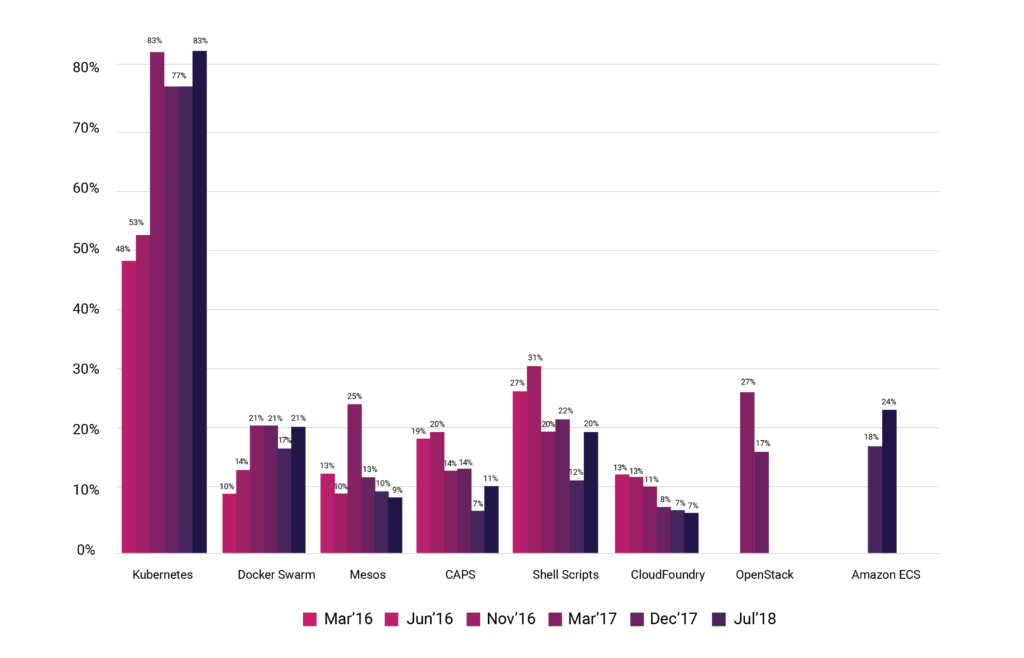
\includegraphics[width=0.8\textwidth]{img/cncf_k8s_survey.png}
\par\end{centering}
\caption{CNCF průzkum využití orchestrátorů, zdroj: \cite{cncf_survey}} \label{fig:cncf_survey}
\end{figure}

\subsection{Souhrn}
Orchestrátory lze porovnávat z mnoha různých úhlů, jako jsou například množství vlastností, nebo kolik dokáží spustit kontejnerů najednou. Nejdůležitější faktorem je však komunita, která se okolo dané technologie pohybuje. Čím větší komunita, tím je nástroj rychleji vyvíjen a je kladen větší důraz na jeho stabilitu. V tomto ohledu jednoznačně dominuje k8s, jenž je nyní brán jako standard pro orchestraci a je běžně součástí komerčních produktů. V současné době má k8s na githubovém repozitáři téměř 52 000 hvězd uživatelů a celkový počet kontributorů do projektu přesáhl 2 100 vývojářů. Je velmi těžké zjistit přesné číslo, kolik firem využívá daný orchestrátor v produkčním prostředí, poskytovatelé cloudů takové statistiky nezveřejňují. Organizace CNCF každoročně pořádá průzkum týkající se Cloudu a kontejnerů, kde je patrné viz obrázek \ref{fig:cncf_survey}, že k8s je nejpopulárnější orchestrátor. V červenci roku 2018 byl třikrát více používanější než konkurenční Docker Swarm. Z tohoto průzkumu také vzešlo, že k8s je nejpoužívanější projekt z CNCF, který je provozován v produkčním nasazení. Proto bude v této práci použit k orchestraci migrované aplikace právě orchestrátor k8s.

\section{Orchestrace workloadu}
K8s je nástroj na provoz a lifecycle kontejnerů, ale sám o sobě neřeší definici a provoz jednotlivých aplikací. Standardní cestou pro vytváření aplikací a objektů v k8s jsou manifesty. Manifest je soubor ve formátu yaml. Přístup a práce s manifesty není složitá, ale s přibývajícím počtem komponent v aplikaci a objektů je velmi obtížné tyto manifesty přehledně udržovat a spravovat. Pro vyřešení tohoto problému bylo zapotřebí vytvořit další úroveň abstrakce nad k8s, která zjednoduší jak verzování, tak provoz aplikací na produkčních clusterech. Celá myšlenka abstrakcí je postavená nad spojování aplikací do funkčních celků, například pokud chce uživatel použít nějakou stávající komponentu, například databázi, nemusí si všechny definice vytvořit sám, ale může použít již částečně hotové řešení. Tato problematika byla řešena v různých projektech s odlišnými řešeními. Nástroje, které tyto operace umožňují používat, by se daly označit jako konfigurační management pro k8s. O zjednodušení zápisu manifestů se opět snaží řada projektů, celkem existuje přes 60 projektů, které se zabývají konfigurováním workloadu. Do výběru byly vybrány projekty s největší komunitou. Správný nástroj by měl splňovat následující požadavky:
\begin{itemize}
    \item \textbf{Deklarativnost} – Nástroj by měl vytvářet konfiguraci, která je jednoznačná a nezávislá na platformě, či závislá na systému \cite{k8s_DAM}.
    \item \textbf{Čitelnost} – Čitelnost předpisu aplikace: manifest jako takový je sice vhodné řešení, ale pokud má aplikace delší list, je snadné se v předpisu ztratit. Definice by měla být lehce čitelná nejen pro stroj, ale i pro člověka.
    \item \textbf{Flexibilita} – Nástroj by měl podporovat několik způsobů užití.
    \item \textbf{Udržovatelnost} – Nástroj by měl být jednoduchý na používání a kód, který je nástrojem vytvořen, by měl být lehce upravitelný a znovupoužitelný.
    \item \textbf{Verzovatelnost} – Ve světě mikroslužeb je nutno posuzovat prostředí a aplikace jako živoucí celek, který se v závislosti na čase mění. Proto je nezbytné uchovávat historii, především z důvodu výpadků a chybám aplikace či clusteru. Podle správného verzování je možné snadno zjistit, kdo v clusteru udělal nějakou změnu a co se stalo předtím, než aplikace přestala správně pracovat.
\end{itemize}

\subsection{Helm}
Helm je projekt, který je často označován jako balíčkovací systém pro k8s, který měl velký vliv na jeho rozšíření. Díky helmu lze velmi jednoduše instalovat aplikace do k8s clusteru. Projekt byl vyvinut firmou Dies, kterou v roce 2017 koupil gigant Microsoft \cite{helm_deis}. Je složen ze dvou hlavních částí, klientská část je označována jako helm a tiller funguje jako serverová část. Tiller běží v k8s a vytváří a řídí aplikace. Právě serverová část helmu vzbuzuje v k8s komunitě velkou kritiku, protože tiller je spouštěn v clusteru s plnými administrátorskými právy. To znamená, že pokud se do clusteru dostane někdo s neoprávněným přístupem, může dojít k ohrožení bezpečnosti chodu k8s clusteru.

\begin{lstlisting}[caption={Kubernetes Manifest - Grafana service, zdroj vlastní},label={lst:helm_temp}]
apiVersion: v1
kind: Service
metadata:
  labels:
    heritage: "{{ .Release.Service }}"
    release: "{{ .Release.Name }}"
    chart: "{{ .Chart.Name }}-{{ .Chart.Version }}"
    app: {{ template "grafana.fullname" . }}
  name: {{ template "grafana.fullname" . }}
{{- if .Values.service.annotations }}
  annotations:
{{ toYaml .Values.service.annotations | indent 4}}
{{- end }}
spec:
  ports:
    - name: http
      port: {{ .Values.port }}
      {{- if eq .Values.service.type "NodePort" }}
      {{- if .Values.service.nodePort }}
      nodePort: {{ .Values.service.nodePort }}
      {{- end -}}
      {{- end }}
  selector:
    app: {{ template "grafana.fullname" . }}
  type: "{{ .Values.service.type }}"
{{- if eq .Values.service.type "LoadBalancer" }}
  {{- if .Values.service.loadBalancerIP }}
  loadBalancerIP: {{ .Values.service.loadBalancerIP }}
  {{- end -}}
  {{- if .Values.service.loadBalancerSourceRanges }}
  loadBalancerSourceRanges:
  {{- range .Values.service.loadBalancerSourceRanges }}
  - {{ . }}
  {{- end }}
  {{- end -}}
{{- end -}}
\end{lstlisting}

Hlavní myšlenkou helmu bylo dodat do k8s stejnou flexibilitu v instalování aplikací, jako tomu je u balíčkovacího systému v Linux. Stačí napsat jeden příkaz a Helm dokáže nainstalovat jakoukoliv aplikaci. Aplikace helmu jsou poté zabaleny do chartu. Chart si lze představit jako yaml šablonu. Vzorovou šablonu (helm šablonu) lze vidět na ukázce kódu číslo \ref{lst:helm_temp}, na ukázce je zobrazena šablona pro k8s službu pro aplikaci Grafana. Díky helmu se dají jednotlivé konfigurační možnosti parametrizovat tak, že pokud je potřeba daný parametr pro aplikaci nastavit, musí být parametrizován. Parametrizování je největší výhoda a zároveň nevýhoda helm šablonování. Jednotlivé charty jsou uloženy v repozitáři, odkud je pak helm instaluje. Helmový repozitář je velmi podobný linuxovému a pracuje s podobnými příkazy jako balíčkovací systém apt. Helm má na GitHubu oficiálně repozitář komunitních helm chartu, ve kterém jsou většinou open source aplikace jako Mariadb, Redis, Tomcat atd. A právě v tomto repozitáři lze najít chart pro Nginx \cite{nginx_helm_template}, z kterého je patrné, jak nepraktické může být šablonování v praxi. Nginx má parametrizovanou většinu svých konfigurovatelných parametrů a než se uživatel v šabloně zorientuje, jaké parametry vlastně potřebuje, bude potřebovat mnohem víc času, než by si napsal vlastní manifest či helm chart. Proto si většinou každá komunita/společnost udržuje vlastní sadu helm chartu, které mají standardizované parametry pro jejich produkční využití.

Většina aktuálních problémů, se kterými se komunita Helmu v současnosti potýká, je spojena právě s komponentou tiller, všechny tyto problémy by měly být vyřešeny v nové verzi Helmu 3 \cite{helm_helm3}. Tato verze ve svém návrhu již nepočítá se serverovou částí a má přidat řadu nových vlastností, jako jsou lepší lifecycle pro aplikace, Lua skriptování atd. Verze Helmu 3 je v současnosti v rané části vývoje a ještě nebylo oznámeno žádné pevné datum, kdy by měla vyjít první stabilní verze.

\subsection{Jsonnet}
U Jsonnetu se nejedná o nástroj na tvorbu manifestů, ale spíše o programovací jazyk. Tento jazyk byl vyvinut Googlem, zpopularizován byl až s nástupem k8s. Jsonnet vychází z klasického JSONu a je rozšířen například o podmínky, cykly, proměnné atd. Díky své velké flexibilitě se stal hned součástí několika nástrojů, jako je Ksonnet, Kubecfg či Kapitan. Obrovskou výhodou je jeho použitelnost při šablonování. Pomocí něho je možno ve velmi krátké době napsat téměř cokoliv. Nevýhodou je složitá syntaxe a operátor bez praxe se jsonnetem jen těžko na první pohled zjistí, co daná šablona dělá.

\begin{lstlisting}[caption={Kapitan komponenta - využívající Jsonnet, zdroj: \cite{kapitan_fleet}},label={lst:kapitan_fleet}]
local kube = import "lib/kube.libjsonnet";
local kap = import "lib/kapitan.libjsonnet";
local inv = kap.inventory();
local server_containers = inv.parameters.gerrit.server.deployment.containers;
local gerrit_pvcs = import "./pvcs.jsonnet";
local gerrit_volume = kube.HostPathVolume(server_containers.gerrit.vol.rev.path)

local gerrit_container = kube.Container("gerrit") {
  image: server_containers.gerrit.image.registry + "/" +
         server_containers.gerrit.image.name + ":" +
         server_containers.gerrit.image.tag,

  volumeMounts: [
  {
    mountPath: "/var/gerrit/review_site",
    name: "reviewsite",
  }],

{
  GerritDeployment(name): kube.Deployment(name) {
    spec+: {
      template+: {
        spec+: {
          containers_+: {
            gerrit: gerrit_container
          },
          volumes_+:{
            reviewsite: gerrit_volume
          },
        },
      },
    },
  },
}
\end{lstlisting}

Na ukázce kódu \ref{lst:kapitan_fleet} je vidět implementace kapitan komponenty postavená na Jsonnetu. Kód uvedený v příkladu lze pomocí kapitan kompilátoru přeložit na k8s manifest. Tento manifest poté obsahuje deployment pro aplikaci Gerrit. V samotném jsonnetu lze používat rozšiřující knihovny. Knihovny jsou napsané v Jsonnetu, mají stejný formát, ale jsou uloženy v souborech označených libsonnet. V uvedeném případě se jedná především o knihovny spojené s k8s objekty. Knihovny jsou nadefinovány pomocí klíčového slova import. Pro zjednodušení a neopakování kódu jsou používány proměnné, které začínají klíčovým slovem local. Například na řádku 8 je vytvořena proměnná \textit{gerrit\_container}, která slouží pro ukládání definice kontejnerové images. Je složena ze třech dalších parametrů, které je možné konfigurovat a přetěžovat, jedná se o parametry kontejnerový repozitář, jméno image a tag. Jednotlivé JSON objekty lze spojovat do vyšších logických celků jako na řádku 20, kde je vytvářen již deployment objekt. Zde je vidět volání funkce z \textit{kube.libsonnet knihovny}. Zápis deployment funkce je strukturou velmi podobný tradičnímu manifestu, na rozdíl od klasického manifestu je možné používat nadefinované proměnné jako výše zmíněný \textit{gerrit\_container}. Jednotlivé JSON bloky jsou propojeny pomocí znaku +.

\subsection{Kustomize}
Kustomize je postaven nad myšlenkou DAM (Declarative Application Management) \cite{k8s_DAM} a je zaměřen na zjednodušení práce s k8s manifesty. Projekt vznikl pod SIG-cli \cite{kustomize_sig} a již od počátku byl vyvíjen tak, aby jeho syntaxe byla co nejbližší ke k8s. Na rozdíl od projektu helm se nejedná o šablonovací jazyk. Kustomize je jednoduchý nástroj na spojování jednotlivých manifestů rozdělených do logických celků. Tyto celky jsou mnohem přehlednější než jeden dlouhý manifest. Nad jednotlivými celky lze jednoduše tvořit úpravy. Základem každé aplikace používající kustomize je kustomomization.yml soubor. V tomto souboru lze nadefinovat cesty manifestů. Kustomomization.yml může jednotlivé parametry v manifestech přepsat. Taková logika funguje i napříč adresáři, je možné například vytvořit adresář base, který bude obsahovat základní aplikaci, a nad ním zadefinovat například další adresáře production a stage, které budou dané manifesty přepisovat. Toto řešení je vhodné především pro vývojáře nebo pro práci více týmů na jedné aplikaci. Další vlastností, kterou lze v kustomize využít, je patch systém. Patche jsou části manifestu, které upravují část původní aplikace. Tyto patche lze jednoduše přidat do Kustomize a ten je při renderování propíše do výsledného manifestu. Ukázku kustomomization souboru je možné sledovat na ukázce kódu číslo \ref{lst:kustomization_yaml}. V příkladu je použit kustomize pro wordpress aplikaci, v sekci base je vidět, že výsledný manifest bude složen ze dvou adresářů, které obsahují další kustomization soubory s manifesty. Dále jsou zde patchesStrategicMerge a vars. První jsou patch, které přepíší hodnoty z base adresářů, a vars poté určuje základní proměnné pro patch soubor. Jednotlivé sestavení výsledného manifestu probíhá pomocí příkazu \textit{kustomize build <cesta na adresář s kustomization.yml>}. Toto je velmi výhodné řešení, pokud do provozu aplikace zasahuje více lidí. Kustomize plně podporuje integraci s gitem, lze tedy nasazovat aplikace přímo z gitu. Projekt je součástí projektů Ship a Argo. Od verze 2.0.3 se stal kustomize součástí nástroje kubectl \cite{kustomize_kubelet}, není proto nutné instalovat žádné rozšiřující nástroje.

\begin{lstlisting}[caption={Kustomization.yml soubor, zdroj: \cite{kustomization_yaml}},label={lst:kustomization_yaml}]
bases:
  - wordpress
  - mysql
patchesStrategicMerge:
  - patch.yaml
namePrefix: demo-

vars:
  - name: WORDPRESS_SERVICE
    objref:
      kind: Service
      name: wordpress
      apiVersion: v1
  - name: MYSQL_SERVICE
    objref:
      kind: Service
      name: mysql
      apiVersion: v1

\end{lstlisting}
\subsection{Kubernetes operátor}
Koncept operátorů je postaven na orchestraci aplikace přímo přes k8s API. V k8s totiž lze využívat objekty zvané CRD (Custome Resource Definition). Pomocí těchto CRD lze rozšířit k8s API o vlastní objekty s vlastní logikou. V praxi to vypadá tak, že v k8s clusteru běží kontejner zvaný operátor, který dokáže nové objekty s nadefinovaným CRD spouštět a vykonávat na nich požadované akce. Operátor nemá žádnou standardizovanou architekturu, jedná se o aplikaci, která komunikuje s k8s API. Aplikace může být napsaná v jakémkoliv jazyce. Pomocí operátoru lze mnohem lépe řešit životní cyklus aplikace, lze prostřednictvím něj sledovat stav jednotlivých zdrojů v clusteru a na základě změn reagovat v aplikaci. S vývojem konceptu operátor začala především firma CoreOS, která napsala základní funkcionalitu a otevřela zdrojové kódy pro nástroj zvaný operator-sdk. Tento nástroj slouží k psaní operátorů. Sdk je dostupné pouze pro programovací jazyk go. Nástroj zjednodušuje především vytvoření nových k8s API a controlleru pro nové objekty, zároveň lze pomocí něj generovat boilerplate kód. Princip operátorů se používá převážně u větších aplikací a systémů, kde je nutné kombinovat více faktorů dohromady, například před upgradem aplikace je nutnost zálohování, spuštění nových služeb a podobně. Nevýhodou oproti ostatním řešením může být složitost implementace operátoru. Operátor nelze nastavovat pouze změnou yamlů, logiku celého operátoru je nutné naprogramovat.

\begin{figure}[H]
\begin{centering}
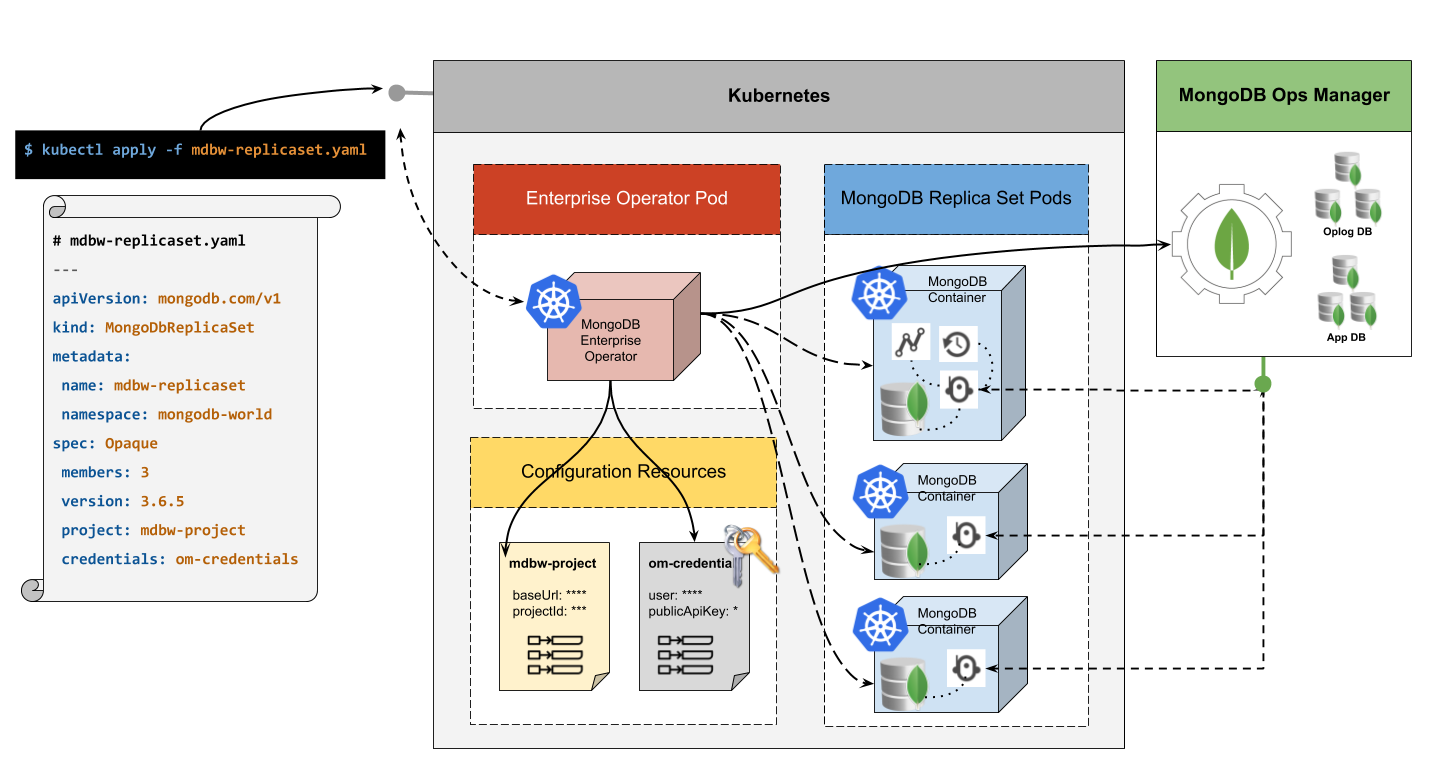
\includegraphics[width=1\textwidth]{img/operator_schema.png}
\par\end{centering}
\caption{Schéma MongoDB Enterprise operátoru, zdroj:\cite{operator_mongodb}} \label{fig:operator_schema}
\end{figure}

Na obrázku \ref{fig:operator_schema} je vidět schéma Kubernetes operátoru pro aplikaci MongoDB. Dále je zde patrné, jak funguje komunikace v rámci operátoru. Operátor je spuštěn jako kontejner běžící v Kubertnetes clusteru, ten dokáže číst CRD. Příklad CRD je v levé části obrázku, jedná se o objekt MongoDbReplicaSet. Operátor dokáže tento k8s objekt rozpoznat a vykonat akce, které jsou v logice operátoru popsány. Samotný MongoDB operátor se v tomto případě nestará pouze o instalaci, ale o celý životní cyklus databáze, operátor totiž dokáže komunikovat i s MongoDB Ops Managerem. Tato aplikace slouží k ovládání životního cyklu aplikace, pomocí manageru lze řešit automatizaci, zálohy či monitoring databáze. Součástí podů je kromě volume a databáze i ops agent, který slouží ke komunikaci mezi jednotlivými databázemi a Ops managerem.

\subsection{Srovnání}
Z následujícího přehledu lze vyvodit, že neexistuje žádný nejlepší přístup k orchestraci workloadu. Žádné z řešení není univerzální, každé má své výhody a nevýhody a je určeno ke specifickému užití. Helm se nejspíše díky své jednoduchosti udrží jako nejpoužívanější balíčkovací manager, nástroje postavené nad jsonnetem zde budou pro pokročilejší uživatele. Kustomize působí jako vyplnění pro stávající manifestová řešení, například je součástí projektu Ship, kde pomocí kustomizem lze upravovat Helm charty. Operátory zde zůstávají jako alternativa pro komplexní aplikace, které potřebují pro svoji orchestraci komplikovanější logiku. Nutno zmínit, že toto srovnání se týká nástrojů v současné době, všechny nástroje se rychle vyvíjejí a je jen těžko odhadnutelné, jakým směrem a způsobem se bude vývoj přístupu k orchestraci workloadu ubírat v dalších letech.
